\documentclass[11pt,a4paper]{article}
\usepackage[utf8]{inputenc}
\usepackage[vietnamese]{babel}
\usepackage{amsmath,amssymb}
\usepackage[version=4]{mhchem}
\usepackage{geometry}
\geometry{top=0.65cm,bottom=0.65cm,left=1.25cm,right=1.25cm,headheight=20pt,headsep=3pt,footskip=9pt}
\usepackage{graphicx}
\usepackage{xcolor}
\usepackage{tabularx}
\usepackage{array}
\usepackage{tikz}
\usepackage{multicol}
\usepackage{fancyhdr}
\usepackage{enumitem}

\definecolor{hfRed}{HTML}{D32F2F}
\definecolor{hfGreen}{HTML}{8BC390}
\definecolor{mainGreen}{HTML}{2E7D32}

\usepackage{ex_test}

\pagestyle{fancy}
\fancyhf{}
\renewcommand{\headrulewidth}{0.75pt}
\renewcommand{\headrule}{\hbox to\headwidth{\color{hfGreen}\leaders\hrule height \headrulewidth\hfill}}
\renewcommand{\footrulewidth}{0.75pt}
\renewcommand{\footrule}{\hbox to\headwidth{\color{hfGreen}\leaders\hrule height \footrulewidth\hfill}}

\fancyhead[L]{\small\itshape\color{hfRed}Tài liệu lưu hành nội bộ}
\fancyhead[R]{\small\color{hfRed}Thầy \textbf{TRẦN VĂN THẠNH} - 0777.470.803}

\fancyfoot[L]{\footnotesize\itshape\color{hfRed}CS1: 6/15 Nguyễn Hoàng, P. Kim Long, TP Huế \quad|\quad CS2: 24 Đặng Thái Thân, TP Huế}
\fancyfoot[R]{\small\textbf{\color{hfRed}Trang \thepage}}

\setlength{\parindent}{0pt}
\setlength{\parskip}{1.0pt}

\def\loigiai#1{
\par\begingroup\color{blue!80!black}\small
\noindent\textbf{\textit{Lời giải chi tiết:}}\par
#1\par\endgroup}

\begin{document}
\Opensolutionfile{ans}[ans-de20-gv]

\noindent
\begin{minipage}[t]{0.48\textwidth}
	\textbf{SỞ GIÁO DỤC VÀ ĐÀO TẠO THỪA THIÊN HUẾ}\\
	\textbf{TRƯỜNG THPT HAI BÀ TRƯNG}\\
	\textbf{ĐỀ CHÍNH THỨC}\\
	\textit{(Đề thi có 04 trang)}
\end{minipage}\hfill
\begin{minipage}[t]{0.48\textwidth}
	\raggedleft
	\textbf{\color{mainGreen}ĐỀ KIỂM TRA ĐỊNH KỲ CHƯƠNG 7 (KIM LOẠI NHÓM IA \& IIA)}\\
	\textbf{MÔN: HOÁ HỌC -- LỚP 12}\\
	\textit{Thời gian làm bài: 50 phút (không kể thời gian phát đề)}\\
	\textbf{Mã đề thi: 120}
\end{minipage}


\vspace{0.1cm}
\begin{center}
	\textbf{\color{hfRed}\Large (BẢN GIÁO VIÊN -- CÓ LỜI GIẢI CHI TIẾT)}
\end{center}

\vspace{1pt}
\noindent\textit{Họ, tên thí sinh: \dots\dots\dots\dots\dots\dots\dots\dots\dots\dots\dots\dots\dots\dots\dots\dots\dots\dots\dots\dots\dots\dots Lớp: \dots\dots\dots\dots SBD: \dots\dots\dots\dots}\\
\noindent\textit{(Cho biết nguyên tử khối: H = 1; C = 12; N = 14; O = 16; Na = 23; Mg = 24; Al = 27; P = 31; S = 32; Cl = 35,5; K = 39; Ca = 40; Fe = 56; Cu = 64; Zn = 65; Br = 80; Rb = 85,5; Ag = 108; Cs = 133; Ba = 137).}

\vspace{1pt}
\noindent
\textbf{PHẦN I (4,5 điểm -- 18 câu): Câu trắc nghiệm nhiều phương án lựa chọn.}\\
\textit{Thí sinh trả lời từ câu 1 đến câu 18. Mỗi câu hỏi thí sinh chỉ chọn một phương án.}

\begin{ex}
Sodium chloride là gia vị quan trọng trong thức ăn của con người. Công thức của sodium chloride là
\choice
{\ce{NaNO3}.}
{\ce{KNO3}.}
{\True \ce{NaCl}.}
{\ce{KCl}.}
\loigiai{
Sodium chloride có công thức hoá học là \ce{NaCl}.\\
\textbf{Chọn C.}}
\end{ex}

\begin{ex}
Tro thực vật được sử dụng như một loại phân bón cung cấp nguyên tố kali (potassium) cho cây trồng do chứa muối potassium carbonate. Công thức của potassium carbonate là
\choice
{\ce{KCl}.}
{\ce{KOH}.}
{\ce{NaCl}.}
{\True \ce{K2CO3}.}
\loigiai{
Potassium carbonate có công thức hoá học là \ce{K2CO3}.\\
\textbf{Chọn D.}}
\end{ex}

\begin{ex}
Khi nhiệt phân hoàn toàn \ce{NaHCO3} thì sản phẩm của phản ứng nhiệt phân là
\choice
{\ce{NaOH}, \ce{CO2}, \ce{H2}.}
{\ce{Na2O}, \ce{CO2}, \ce{H2O}.}
{\True \ce{Na2CO3}, \ce{CO2}, \ce{H2O}.}
{\ce{NaOH}, \ce{CO2}, \ce{H2O}.}
\loigiai{
$\ce{2NaHCO3 ->[t^\circ] Na2CO3 + CO2 + H2O}$.\\
\textbf{Chọn C.}}
\end{ex}

\begin{ex}
Dãy gồm các kim loại đều phản ứng với nước ở nhiệt độ thường, tạo ra dung dịch có môi trường kiềm là
\choice
{\True Na, Ba, K.}
{Be, Na, Ca.}
{Na, Fe, K.}
{Na, Cr, K.}
\loigiai{
Na, Ba, K phản ứng với nước ở nhiệt độ thường tạo dung dịch base mạnh (kiềm). Be không phản ứng; Fe, Cr không phản ứng với nước ở nhiệt độ thường.\\
\textbf{Chọn A.}}
\end{ex}

\begin{ex}
Cho phương trình hóa học của phản ứng nhiệt phân sau: $\ce{4M(NO3)_{$x$} ->[t^\circ] 2M2O_{$x$} + 4$x$NO2 + $x$O2}$. Kim loại M là
\choice
{Ca.}
{\True Mg.}
{K.}
{Ag.}
\loigiai{
Muối nitrate của các kim loại từ Mg đến Cu khi nhiệt phân tạo basic oxide, \ce{NO2} và \ce{O2}:\\
$\ce{2Mg(NO3)2 ->[t^\circ] 2MgO + 4NO2 + O2}$ (tương ứng $x=2$).\\
\textbf{Chọn B.}}
\end{ex}

\begin{ex}
Cho sơ đồ chuyển hoá hoá học sau:
\par\vspace{1pt}\centerline{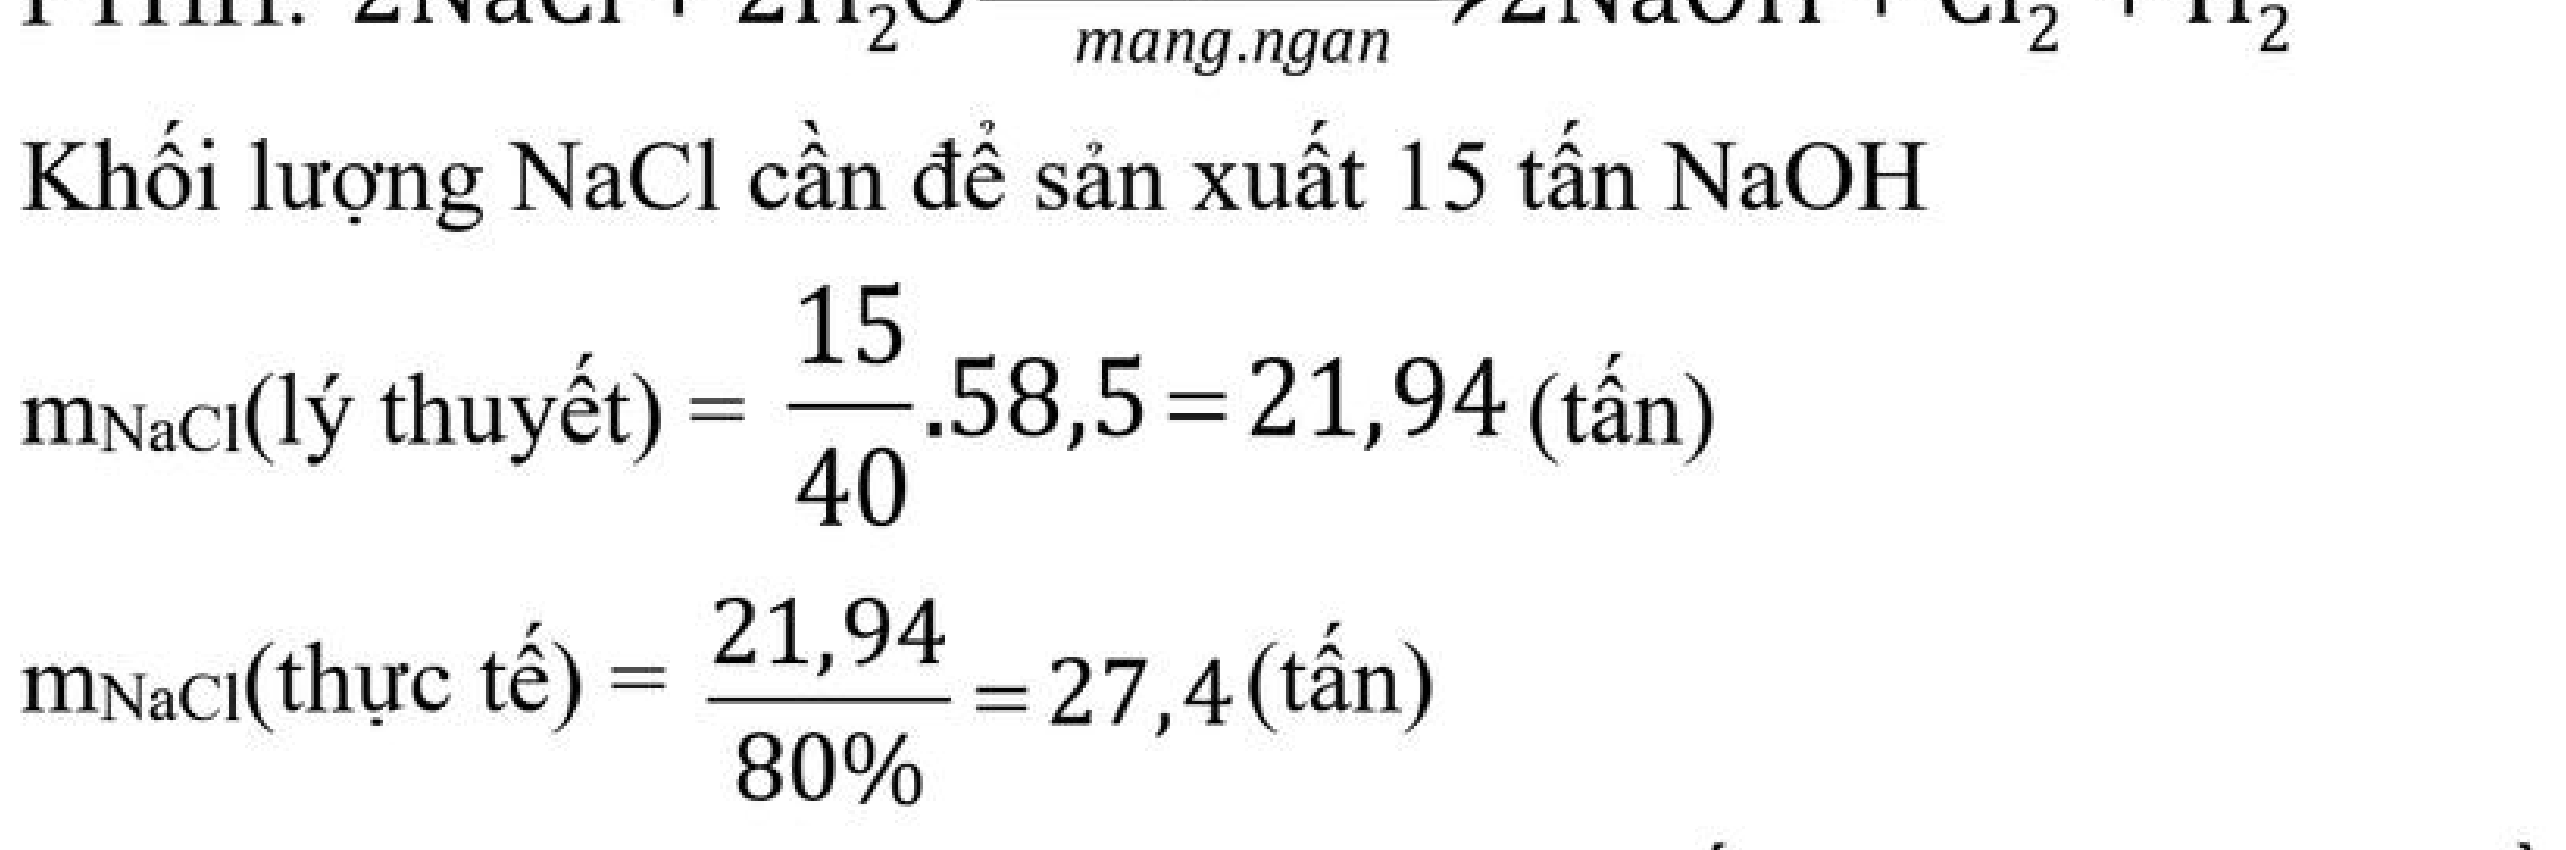
\includegraphics[height=1.45cm]{images_crop_de20/p1_cau6_so_do.png}}\vspace{1pt}
Chất X trong sơ đồ trên có thể là
\choice
{\True \ce{BaCO3}.}
{\ce{CaCO3}.}
{\ce{BaSO3}.}
{\ce{MgCO3}.}
\loigiai{
X là \ce{BaCO3}:\\
-- $\ce{BaCO3 ->[t^\circ] BaO (B_1) + CO2 (A_1)}$.\\
-- $\ce{CO2 + Ca(OH)2 -> CaCO3 v (A_2) + H2O}$; $\ce{CaCO3 ->[900^\circ\text{C}] CaO + CO2}$.\\
-- $\ce{BaO + 2HCl -> BaCl2 (B_2) + H2O}$; $\ce{BaCl2 + Na2SO4 -> BaSO4 v (B_3) + 2NaCl}$.\\
\textbf{Chọn A.}}
\end{ex}

\begin{ex}
Phát biểu nào sau đây \textbf{không} đúng?
\choice
{Đun sôi nước cứng chỉ làm mềm nước cứng tạm thời.}
{Dung dịch \ce{Na2CO3} làm mềm nước cứng tạm thời, nước cứng vĩnh cửu.}
{\True Dung dịch \ce{NH4Cl} làm mềm nước cứng.}
{Cho dung dịch \ce{Ca(OH)2} vừa đủ làm mềm nước cứng tạm thời.}
\loigiai{
Dung dịch \ce{NH4Cl} không kết tủa được \ce{Ca^2+} hay \ce{Mg^2+} nên không làm mềm nước cứng.\\
\textbf{Chọn C.}}
\end{ex}

\begin{ex}
Để xử lí chất thải có tính acid trong công nghiệp và đời sống, người ta thường dùng
\choice
{\True nước vôi.}
{phèn chua.}
{giấm ăn.}
{muối ăn.}
\loigiai{
Nước vôi \ce{Ca(OH)2} có tính kiềm, rẻ tiền và an toàn, dùng để trung hoà tính acid của chất thải: $\ce{H+ + OH- -> H2O}$.\\
\textbf{Chọn A.}}
\end{ex}

\begin{ex}
Hợp chất của calcium nào sau đây \textbf{không} gặp trong tự nhiên ở trạng thái tự do?
\choice
{\ce{CaCO3}.}
{\ce{CaSO4}.}
{\ce{Ca(HCO3)2}.}
{\True \ce{CaO}.}
\loigiai{
\ce{CaO} dễ dàng hút ẩm và tác dụng với hơi nước và \ce{CO2} trong không khí nên không gặp tự do trong tự nhiên.\\
\textbf{Chọn D.}}
\end{ex}



\begin{ex}
Trong các kim loại sau, kim loại nào có tính khử mạnh nhất?
\choice
{\True K.}
{Al.}
{Mg.}
{Na.}
\loigiai{
Potassium (K) thuộc nhóm IA có bán kính lớn hơn Na, tính khử mạnh nhất trong 4 kim loại trên ($E^\circ_{\ce{K+/K}} = -2{,}92\text{ V}$).\\
\textbf{Chọn A.}}
\end{ex}

\begin{ex}
Các dung dịch muối ăn, phèn chua, nước vôi trong được kí hiệu ngẫu nhiên là X, Y, Z. Một số kết quả thí nghiệm được ghi ở bảng sau:\\
-- Mẫu X + dung dịch phenolphthalein $\rightarrow$ Dung dịch chuyển sang màu hồng.\\
-- Mẫu Z + dung dịch \ce{BaCl2} $\rightarrow$ Xuất hiện kết tủa trắng.\\
Các dung dịch ban đầu (muối ăn, phèn chua, nước vôi trong) tương ứng lần lượt với các kí hiệu là
\choice
{\True Y, Z, X.}
{Z, X, Y.}
{X, Y, Z.}
{Y, X, Z.}
\loigiai{
-- X làm phenolphthalein hoá hồng $\rightarrow$ X là nước vôi trong.\\
-- Z tạo kết tủa trắng với \ce{BaCl2} $\rightarrow$ Z là phèn chua (chứa \ce{SO4^2-}).\\
-- Y là muối ăn (NaCl).\\
Thứ tự muối ăn, phèn chua, nước vôi trong là Y, Z, X.\\
\textbf{Chọn A.}}
\end{ex}

\begin{ex}
Nguyên tố kim loại nhóm IIA được tìm thấy trong tự nhiên dưới dạng nào sau đây?\\
(1) Các cation $\ce{M^2+}$ trong nước sông, hồ, nước ngầm, nước biển.\\
(2) Các khoáng vật ít tan như carbonate, sulfate, silicate.\\
(3) Các hợp chất ít tan cấu tạo nên răng, xương động vật.
\choice
{(1) và (2).}
{(1) và (3).}
{\True (1), (2) và (3).}
{(2) và (3).}
\loigiai{
Cả 3 dạng trên đều là dạng tồn tại tự nhiên của các nguyên tố kim loại nhóm IIA.\\
\textbf{Chọn C.}}
\end{ex}

\begin{ex}
Barium phản ứng với nước dễ dàng hơn nhiều so với magnesium ở điều kiện thường là do các nguyên nhân nào sau đây?\\
(1) Barium có tính khử mạnh hơn magnesium.\\
(2) Độ tan của barium hydroxide trong nước cao hơn nhiều so với magnesium hydroxide.\\
(3) Bọt khí hydrogen sinh ra bám trên bề mặt magnesium nhiều hơn, cản trở phản ứng tiếp diễn.
\choice
{(1).}
{(1), (2) và (3).}
{(1) và (3).}
{\True (1) và (2).}
\loigiai{
(1) Đúng do Ba có tính khử mạnh hơn Mg; (2) Đúng do \ce{Ba(OH)2} tan tốt giải phóng bề mặt kim loại liên tục. (3) không phải là nguyên nhân chính.\\
\textbf{Chọn D.}}
\end{ex}

\begin{ex}
Nhiệt độ phân huỷ thành oxide của các muối carbonate của kim loại nhóm IIA giảm dần theo dãy nào sau đây?
\choice
{\ce{MgCO3}, \ce{CaCO3}, \ce{SrCO3}, \ce{BaCO3}.}
{\True \ce{BaCO3}, \ce{SrCO3}, \ce{CaCO3}, \ce{MgCO3}.}
{\ce{BaCO3}, \ce{CaCO3}, \ce{SrCO3}, \ce{MgCO3}.}
{\ce{MgCO3}, \ce{BaCO3}, \ce{SrCO3}, \ce{CaCO3}.}
\loigiai{
Độ bền nhiệt tăng dần từ \ce{MgCO3} đến \ce{BaCO3}, do đó nhiệt độ phân huỷ giảm dần theo thứ tự: $\ce{BaCO3 > SrCO3 > CaCO3 > MgCO3}$.\\
\textbf{Chọn B.}}
\end{ex}

\begin{ex}
Dãy các kim loại nào sau đây tác dụng nhanh với nước ở điều kiện thường?
\choice
{Be, Na, Ba.}
{Mg, Ca, Ba.}
{\True Li, Ca, Ba.}
{Sr, Sn, Ba.}
\loigiai{
Li, Ca, Ba đều phản ứng nhanh mãnh liệt với nước ở nhiệt độ thường. Be trơ; Mg phản ứng rất chậm; Sn không tan trong nước.\\
\textbf{Chọn C.}}
\end{ex}

\begin{ex}
Ion $\ce{Ca^2+}$ ($Z = 20$) đóng vai trò thiết yếu trong việc phát triển xương, giúp duy trì hoạt động của cơ bắp, kích thích máu lưu thông, điều tiết một số loại hormone,... Tổng số hạt proton và electron của ion $\ce{Ca^2+}$ là
\choice
{40.}
{42.}
{\True 38.}
{18.}
\loigiai{
Ion $\ce{Ca^2+}$ có 20 proton và $20 - 2 = 18$ electron. Tổng số hạt proton và electron = $20 + 18 = 38$.\\
\textbf{Chọn C.}}
\end{ex}

\begin{ex}
Đặc điểm nào sau đây là đặc điểm chung của nước có tính cứng vĩnh cửu và nước có tính cứng toàn phần?
\choice
{\True Đều có thể làm mềm bằng dung dịch \ce{Na3PO4}.}
{Đều không chứa anion \ce{HCO3-}.}
{Đều bị mất một phần tính cứng khi đun sôi nước.}
{Thành phần anion hoàn toàn giống nhau.}
\loigiai{
Dung dịch \ce{Na3PO4} tạo kết tủa phosphat với \ce{Ca^2+}, \ce{Mg^2+} làm mềm cả nước cứng vĩnh cửu và toàn phần.\\
\textbf{Chọn A.}}
\end{ex}

\begin{ex}
Cho các phát biểu sau:\\
(a) Tất cả các kim loại kiềm thổ đều tan trong nước ở nhiệt độ thường.\\
(b) Các kim loại kiềm có thể đẩy được kim loại yếu hơn ra khỏi dung dịch muối của chúng.\\
(c) Các ion $\ce{Na+}$, $\ce{Mg^2+}$, $\ce{Al^3+}$ có cùng cấu hình electron ở trạng thái cơ bản và đều có tính oxi hoá yếu.\\
(d) Các kim loại kiềm K, Rb, Cs tự bốc cháy khi tiếp xúc với nước.\\
(e) Kim loại magnesium có cấu trúc mạng tinh thể lục phương.\\
Trong các phát biểu trên, số phát biểu đúng là
\choice
{2.}
{\True 3.}
{4.}
{5.}
\loigiai{
Có 3 phát biểu đúng là (c), (d), (e). (a) sai vì Be không tan, Mg tan rất chậm; (b) sai vì kim loại kiềm tác dụng với nước trước.\\
\textbf{Chọn B.}}
\end{ex}



\noindent
\textbf{PHẦN II (4,0 điểm -- 4 câu): Câu trắc nghiệm đúng sai.}\\
\textit{Thí sinh trả lời từ câu 1 đến câu 4. Trong mỗi ý a), b), c), d) ở mỗi câu, thí sinh chọn đúng hoặc sai.}

\setcounter{ex}{0}

\begin{ex}
Mỗi phát biểu sau đây về hợp chất của sodium là đúng hay sai?
\par\vspace{1pt}\centerline{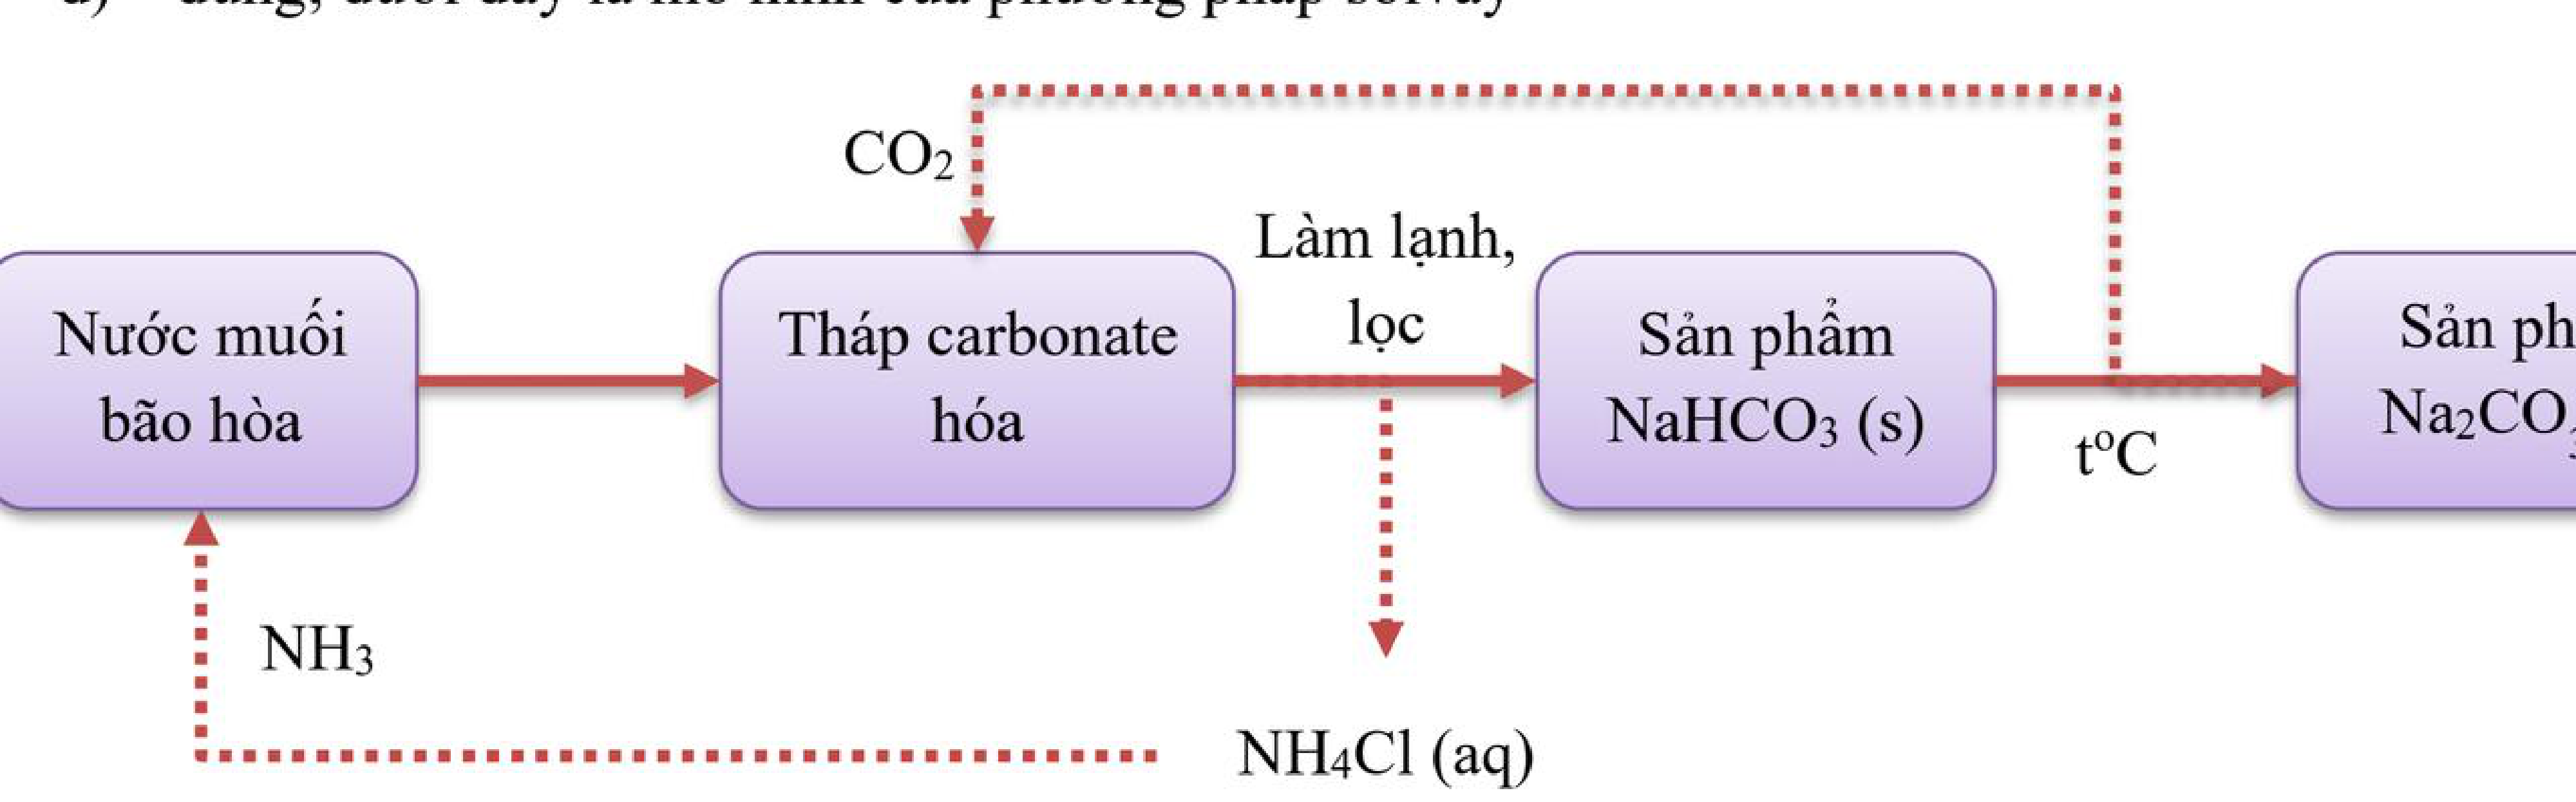
\includegraphics[height=2.3cm]{images_crop_de20/p2_cau1_solvay.png}}\vspace{1pt}
\choiceTF
{Điện phân dung dịch \ce{NaCl} có màng ngăn xốp thu được \ce{NaOH}, \ce{H2} và \ce{O2}.}
{\True \ce{NaHCO3} là hợp chất lưỡng tính.}
{\True \ce{Na2CO3} là nguyên liệu quan trọng để sản xuất thuỷ tinh.}
{\True Phương pháp Solvay sản xuất \ce{NaHCO3} từ nguyên liệu chính là \ce{NH3}, \ce{NaCl} và \ce{CO2}.}
\loigiai{
a) \textbf{Sai}. Điện phân dung dịch \ce{NaCl} có màng ngăn thu được \ce{Cl2} ở anode, \ce{H2} và \ce{NaOH} ở cathode.\\
b) \textbf{Đúng}. \ce{NaHCO3} vừa tác dụng với acid vừa tác dụng với base.\\
c) \textbf{Đúng}. Soda \ce{Na2CO3} là nguyên liệu nấu chảy thuỷ tinh.\\
d) \textbf{Đúng}. Phương pháp Solvay dùng \ce{NaCl}, \ce{NH3}, \ce{CO2} và \ce{H2O} tạo \ce{NaHCO3} kết tủa.}
\end{ex}

\begin{ex}
Sodium chloride là một hợp chất ion điển hình.
\choiceTF
{\True Ở trạng thái nóng chảy, sodium chloride có khả năng dẫn điện.}
{\True Sodium chloride có nhiệt độ nóng chảy cao.}
{Trong tinh thể sodium chloride ở điều kiện thường, các ion có thể di chuyển tự do.}
{Khi dùng búa đập vào hạt muối thì hạt muối bị biến dạng do có tính dẻo.}
\loigiai{
a) \textbf{Đúng}. Ở trạng thái nóng chảy, các ion \ce{Na+} và \ce{Cl-} chuyển động tự do dẫn điện.\\
b) \textbf{Đúng}. Lực hút tĩnh điện giữa các ion rất mạnh nên \ce{NaCl} có nhiệt độ nóng chảy cao ($801^\circ\text{C}$).\\
c) \textbf{Sai}. Ở trạng thái rắn, các ion nằm ở vị trí cố định nút mạng.\\
d) \textbf{Sai}. Muối ăn có tính giòn, đập vào sẽ vỡ vụn.}
\end{ex}

\begin{ex}
Mỗi phát biểu sau đây về kim loại kiềm thổ là đúng hay sai?
\choiceTF
{Các oxide của kim loại kiềm thổ đều bị khí CO khử thành kim loại tự do ở nhiệt độ cao.}
{\True Các kim loại Ca, Mg và Ba chỉ điều chế được bằng phương pháp điện phân nóng chảy.}
{Các kim loại Mg và Ba đều khử được ion \ce{Ag+} trong dung dịch thành Ag.}
{\True Cho kim loại Mg vào dung dịch \ce{FeCl3} dư thì không thu được kim loại Fe.}
\loigiai{
a) \textbf{Sai}. Khí CO không khử được oxide kim loại kiềm thổ.\\
b) \textbf{Đúng}. Do tính khử rất mạnh, Ca, Mg, Ba chỉ điều chế bằng điện phân nóng chảy.\\
c) \textbf{Sai}. Ba tác dụng với nước trước trong dung dịch.\\
d) \textbf{Đúng}. Do $\ce{FeCl3}$ dư nên Mg hết: $\ce{Mg + 2FeCl3 -> MgCl2 + 2FeCl2}$.}
\end{ex}

\begin{ex}
Hợp chất của kim loại kiềm có nhiều ứng dụng quan trọng trong thực tiễn.
\choiceTF
{\True Sodium carbonate khan (\ce{Na2CO3}, còn gọi là soda) được dùng trong công nghiệp thuỷ tinh, đồ gốm, bột giặt,...}
{\True Sodium hydrogencarbonate (\ce{NaHCO3}) được dùng trong công nghiệp thực phẩm làm bột nở và dùng làm thuốc giảm đau dạ dày.}
{\True Dung dịch \ce{NaCl} có nồng độ 0,9\% (nước muối sinh lý) được dùng để vệ sinh, súc miệng và sát khuẩn.}
{Chất thường được gọi là xút ăn da là KOH.}
\loigiai{
a) \textbf{Đúng}. Soda dùng trong công nghiệp luyện thuỷ tinh, gốm sứ, xà phòng.\\
b) \textbf{Đúng}. Bột nở làm bánh và trung hoà acid dạ dày.\\
c) \textbf{Đúng}. Nước muối sinh lý 0,9\%.\\
d) \textbf{Sai}. Xút ăn da là NaOH, KOH là potash ăn da.}
\end{ex}



\noindent
\textbf{PHẦN III (1,5 điểm -- 6 câu): Câu trắc nghiệm yêu cầu trả lời ngắn.}\\
\textit{Thí sinh trả lời từ câu 1 đến câu 6.}

\setcounter{ex}{0}

\begin{ex}
Cho các phát biểu sau:\\
(1) Nhúng đầu dây inox sạch vào dung dịch muối \ce{NaCl} rồi đưa vào ngọn lửa đèn khí thấy ngọn lửa nhuộm màu vàng tươi.\\
(2) Muối potassium carbonate tan tốt trong nước.\\
(3) Trong công nghiệp, một lượng lớn soda được dùng để sản xuất thuỷ tinh.\\
(4) Sodium hydrogencarbonate là chất rắn màu trắng, bền ở nhiệt độ thường.\\
(5) Điện phân dung dịch \ce{NaCl} có màng ngăn xốp thì ở cathode thu được kim loại Na.\\
Có bao nhiêu phát biểu đúng trong các phát biểu trên?
\par\noindent\textbf{Đáp số:} \textbf{\color{red}4}
\loigiai{
Có 4 phát biểu đúng là (1), (2), (3), (4). (5) sai vì ở cathode thu được khí \ce{H2} và \ce{NaOH}.\\
\textbf{Đáp số: 4.}}
\end{ex}

\begin{ex}
Baking soda bị phân huỷ khi đun nóng tạo thành soda, khí carbon dioxide và hơi nước. Tổng hệ số nguyên tối giản của các chất trong phương trình hoá học của phản ứng nhiệt phân baking soda là bao nhiêu?
\par\noindent\textbf{Đáp số:} \textbf{\color{red}5}
\loigiai{
$\ce{2NaHCO3 ->[t^\circ] Na2CO3 + CO2 + H2O}$.\\
Tổng hệ số tối giản = $2 + 1 + 1 + 1 = 5$.\\
\textbf{Đáp số: 5.}}
\end{ex}

\begin{ex}
Cho dãy các kim loại: Fe, Na, Ba, Ca. Có bao nhiêu kim loại trong dãy trên tác dụng được với nước ở nhiệt độ thường?
\par\noindent\textbf{Đáp số:} \textbf{\color{red}3}
\loigiai{
Có 3 kim loại là Na, Ba, Ca. Fe không tác dụng với nước ở nhiệt độ thường.\\
\textbf{Đáp số: 3.}}
\end{ex}

\begin{ex}
Có bao nhiêu chất bị phân huỷ bởi nhiệt độ trong dãy các chất sau: \ce{Na2CO3}, \ce{BaCO3}, \ce{CaSO4}, \ce{Ca(HCO3)2}, \ce{Mg(NO3)2}, \ce{NaHCO3}?
\par\noindent\textbf{Đáp số:} \textbf{\color{red}4}
\loigiai{
Có 4 chất bị nhiệt phân: \ce{BaCO3}, \ce{Ca(HCO3)2}, \ce{Mg(NO3)2}, \ce{NaHCO3}.\\
\ce{Na2CO3} và \ce{CaSO4} bền nhiệt.\\
\textbf{Đáp số: 4.}}
\end{ex}

\begin{ex}
Ở điều kiện thường, kim loại calcium (Ca) kết tinh theo mạng tinh thể lập phương tâm diện với khối lượng riêng thực nghiệm $D = 1{,}55\text{ g/cm}^3$. Giả thiết các nguyên tử Ca là những hình cầu chiếm 74\% thể tích tinh thể, phần còn lại là các khe rỗng. Cho biết thể tích hình cầu $V = \frac{4}{3}\pi r^3$; số Avogadro $N_A = 6{,}023\times 10^{23}\text{ mol}^{-1}$; số $\pi = 3{,}1416$; khối lượng mol của Ca là $40\text{ g/mol}$. Tính bán kính nguyên tử Ca theo đơn vị picomet (pm) (làm tròn kết quả đến phần nguyên).
\par\noindent\textbf{Đáp số:} \textbf{\color{red}196}
\loigiai{
Thể tích 1 mol tinh thể: $V_{\text{tt}} = \dfrac{40}{1{,}55} \approx 25{,}80645\text{ cm}^3$.\\
Thể tích nguyên tử Ca: $V_{\text{nt}} = 25{,}80645 \times 0{,}74 \approx 19{,}09677\text{ cm}^3$.\\
Thể tích 1 nguyên tử: $V_1 = \dfrac{19{,}09677}{6{,}023\times 10^{23}} \approx 3{,}1706\times 10^{-23}\text{ cm}^3$.\\
Bán kính: $r = \sqrt[3]{\dfrac{3V_1}{4\pi}} \approx 1{,}9634\times 10^{-8}\text{ cm} = 196{,}34\text{ pm} \approx 196\text{ pm}$.\\
\textbf{Đáp số: 196.}}
\end{ex}

\begin{ex}
Khi điện phân 500 mL dung dịch \ce{NaCl} với điện cực trơ, có màng ngăn xốp đến khi khối lượng dung dịch giảm 5,475 gam thì ngừng điện phân, thu được dung dịch X (coi thể tích dung dịch thay đổi không đáng kể và nước bay hơi không đáng kể). Xác định giá trị pH của dung dịch X (làm tròn kết quả đến hai chữ số thập phân).
\par\noindent\textbf{Đáp số:} \textbf{\color{red}13,48}
\loigiai{
$\ce{2NaCl + 2H2O -> 2NaOH + Cl2 + H2}$\\
Gọi $x$ là số mol \ce{NaCl} phản ứng:\\
$m_{\text{giảm}} = m_{\ce{Cl2}} + m_{\ce{H2}} = 71 \times 0{,}5x + 2 \times 0{,}5x = 36{,}5x = 5{,}475\text{ g} \rightarrow x = 0{,}15\text{ mol}$.\\
$n_{\ce{NaOH}} = 0{,}15\text{ mol} \rightarrow [\ce{OH-}] = \dfrac{0{,}15}{0{,}5} = 0{,}3\text{ M}$.\\
$\text{pOH} = -\log(0{,}3) \approx 0{,}52288 \rightarrow \text{pH} = 14 - 0{,}52288 \approx 13{,}48$.\\
\textbf{Đáp số: 13,48.}}
\end{ex}

\vspace{0.3cm}
\noindent
\textbf{\color{hfRed}\large BẢNG ĐÁP ÁN THAM KHẢO TOÀN ĐỀ}

\vspace{0.1cm}
\noindent
\textbf{\color{mainGreen}PHẦN I:} 1.C \quad 2.D \quad 3.C \quad 4.A \quad 5.B \quad 6.A \quad 7.C \quad 8.A \quad 9.D \quad 10.A \quad 11.A \quad 12.C \quad 13.D \quad 14.B \quad 15.C \quad 16.C \quad 17.A \quad 18.B

\vspace{0.1cm}
\noindent
\textbf{\color{mainGreen}PHẦN II:} Câu 1: a-S, b-Đ, c-Đ, d-Đ \quad|\quad Câu 2: a-Đ, b-Đ, c-S, d-S\\
Câu 3: a-S, b-Đ, c-S, d-Đ \quad|\quad Câu 4: a-Đ, b-Đ, c-Đ, d-S

\vspace{0.1cm}
\noindent
\textbf{\color{mainGreen}PHẦN III:} Câu 1: \textbf{4} \quad|\quad Câu 2: \textbf{5} \quad|\quad Câu 3: \textbf{3} \quad|\quad Câu 4: \textbf{4} \quad|\quad Câu 5: \textbf{196} \quad|\quad Câu 6: \textbf{13,48}

\Closesolutionfile{ans}
\end{document}
